% !TeX root = these.tex
\section{Les outils partie serveur}


\subsection{Java EE}

%% ce paragraphe est un copié-collé de commentCaMarche et est, forcement à retravailler
La plateforme Java entreprise (Java EE) est un ensemble de spécifications portée par un consortium de sociétés internationales qui permettent ensemble des solutions pour le développement, le déploiement, et de la gestion des applications d'entreprises multi-niveaux, basées sur des composants.

\begin{figure}[!h]
    \center
   	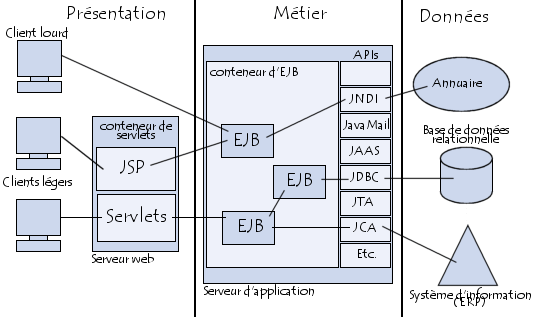
\includegraphics[scale=0.65]{architecture_JEE.png}
   	\caption{Diagramme issu de\url{architecture_JEE.png}}
    \label{reference1}
\end{figure}

Et dans la figure  \ref{reference1}\footnote{Diagramme issu de \url{}}
** image**
Construit sur la plateforme de Java 2 édition standard (Java SE), la plateforme Java EE ajoute les possibilités nécessaires pour fournir une plateforme complète, stable, sécurisée, et rapide de Java au niveau entreprise. 
Dans la mesure où J2EE s'appuie entièrement sur le Java, il bénéficie des avantages et inconvénients de ce langage, en particulier une bonne portabilité et une maintenabilité du code.\\
\newline
\indent
L'ensemble de l'infrastructure d'execution JavaEE est donc constitué de services (API) et spécifications tel que:
HTTP et HTTPS
Java Transaction API (JTA)
Remote Method Invocation/Internet Inter-ORB Protocol (RMI/IIOP)
Java Interface Definition Language (Java IDL)
Java DataBase Connectivity (JDBC)
Java Message Service (JMS)
Java Naming and Directory Interface (JNDI)
API JavaMail et JAF (JavaBeans Activation Framework)
Java API for XML Processing (JAXP)
Java EE Connector Architecture
Gestionnaires de ressources
Entreprise Java Beans (EJB)
Java Server Pages (JSP)
Servlet
Java API for XML Web Services (JAX-WS, anciennement JAX-RPC)
SOAP with Attachments API for Java (SAAJ)
Java API for XML Registries (JAXR)

Dans le cadre de notre application, seule une sous partie de ces composants nous ont été utile, tel que, notemment, les servelets, les JSP, JavaMail ou encore Jdbc avec hibernate, tel que décrit dans le point suivant.

De plus, l'architecture J2EE repose sur des composants distincts, interchangeables et distribués, ce qui signifie notamment :

qu'il est simple d'étendre l'architecture ;
qu'un système reposant sur J2EE peut posséder des mécanismes de haute-disponibilité, afin de garantir une bonne qualité de service ;
que la maintenabilité des applications est facilitée.

Pour interagir avec notre solveur d'une part, de la base de données d'autre part, et par


%% ==== avantages
java EE vs php vs .net vs python

%% === apprentissage
Ce fut nouveau mais xxx
Ca nous à permit d'apprender les outils et les techniques les plus recherchée actuelement 

\subsection{Hibernate}

Pour pouvoir communiquer avec notre base de donnée à partir de notre code java, on a commencé avec jdbc\footnote{Java Database connectivity} mais cela n'était pas suffisant et on s'est tourné ver Hibernate.

Hibernate est un framework libre, appellé framework de  "mapping objet-relationnel" ou encore de "persistance objet des données" (voir Figure \ref{reference2}). 
\begin{figure}[!h]
    \center
   	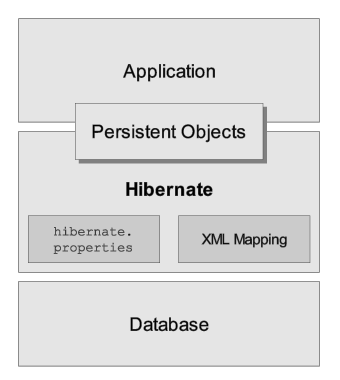
\includegraphics[scale=0.65]{schema_hibernate.png}
   	\caption{Diagramme issu de\url{}}
    \label{reference2}
\end{figure}
Ca permet donc à la couche applicative de notre programme de traiter les données vennant de la base de donnée comme des objects donc le contenu reste en mémoire même après la fin d'exécution du programme. D'où persistance objet des données. Le lien entre les classes exposées et la source physique des données (dans notre cas une base de données *relationnelle*) est définie par un fichier xml. D'où mapping objet-relationnel.
Cela nous à permit de gérer notre base de données, comme le reste de l'application en orienté objet, et même si son apprentissage ne fut pas des plus aisée, la gestion générale du code s'en est retrouvé grandement amélioré.

Un autre avantage recherché par cette solution, est que son indépendance à la base de donnée le rend ultra portable, et, sans aucune modification du code, notre application peu tourner sur 221\footnote{http://developers.sun.com/product/jdbc/drivers} base de données différente.  Notre application, après avoir configuré ses crédential dans le fichier de configuration d'Hibernate, se chargera de créer l'entièretée des tables et la structure de la base de donnée.

Théoriquement il aurait donc été possible d'envoyer directement un objet "hibernate" (représentant par exemple une table de notre bdd), à gwt, donc à l'utilisateur, malheureusement le monde n'est pas parfait, et comme stipulé dans la doc GWT\footnote{https://developers.google.com/web-toolkit/articles/using\_gwt\_with\_hibernate},
une SerializationException est levée à chaque fois un type transférée sur RPC n'est pas «sérialisable». La définition de la sérialisibilité signifie ici que le mécanisme RPC GWT sait comment sérialiser et désérialiser le type de bytecode au format JSON et vice-versa.
Le problème vient du fait qu'Hibernate modifie les objects afin de les rendre persistant (pour être exact, c'est la librairie javassist qui se charge de réécrire le bytecode de ces objects pour les rendre persistant). Au moment du transfer de l'object, une serialisation est tantée, mais n'étant pas le même (car modifé par javassist), il ne peut être sérialisé par RPC-GWTP.
Il a fallut donc rajouter des classes de type DTO\footnote{Data Transfer Object}, qui, eu sérialisable ont pu servir de communiquation entre la partie cliente et serveur.

Hibernate possedant sont propre language de requète HQL \footnote{Hibernate Query Language}, d'apparence similaire au SQL, mais pleinement orienté Object et comprenant des notions comme l'inheritance ou le polymorphisme\footnote{https://docs.jboss.org/hibernate/orm/3.3/reference/en/html/queryhql.html}.  Mais ca nous à bien fais chier (xx), et on a pas su en tirer pleinement avantage.

